\documentclass[tikz,border=8pt]{standalone}
\usepackage[T1]{fontenc}
\usepackage{lmodern}
\usepackage{xcolor}
\usetikzlibrary{arrows.meta,positioning,fit,calc}

\definecolor{ink}{HTML}{1F1F1F}
\definecolor{muted}{HTML}{666666}
\definecolor{bluefill}{HTML}{EAF2FF}
\definecolor{blueline}{HTML}{1F74FF}
\definecolor{gatefill}{HTML}{FFF8E8}
\definecolor{gateline}{HTML}{D58B00}
\definecolor{passfill}{HTML}{E8F7EF}
\definecolor{passline}{HTML}{00A65A}
\definecolor{pausefill}{HTML}{FFF1D7}
\definecolor{denyfill}{HTML}{FDE8E8}
\definecolor{denyline}{HTML}{E13D3D}
\definecolor{softgray}{HTML}{F7F7F7}
\definecolor{grayline}{HTML}{BDBDBD}

\begin{document}
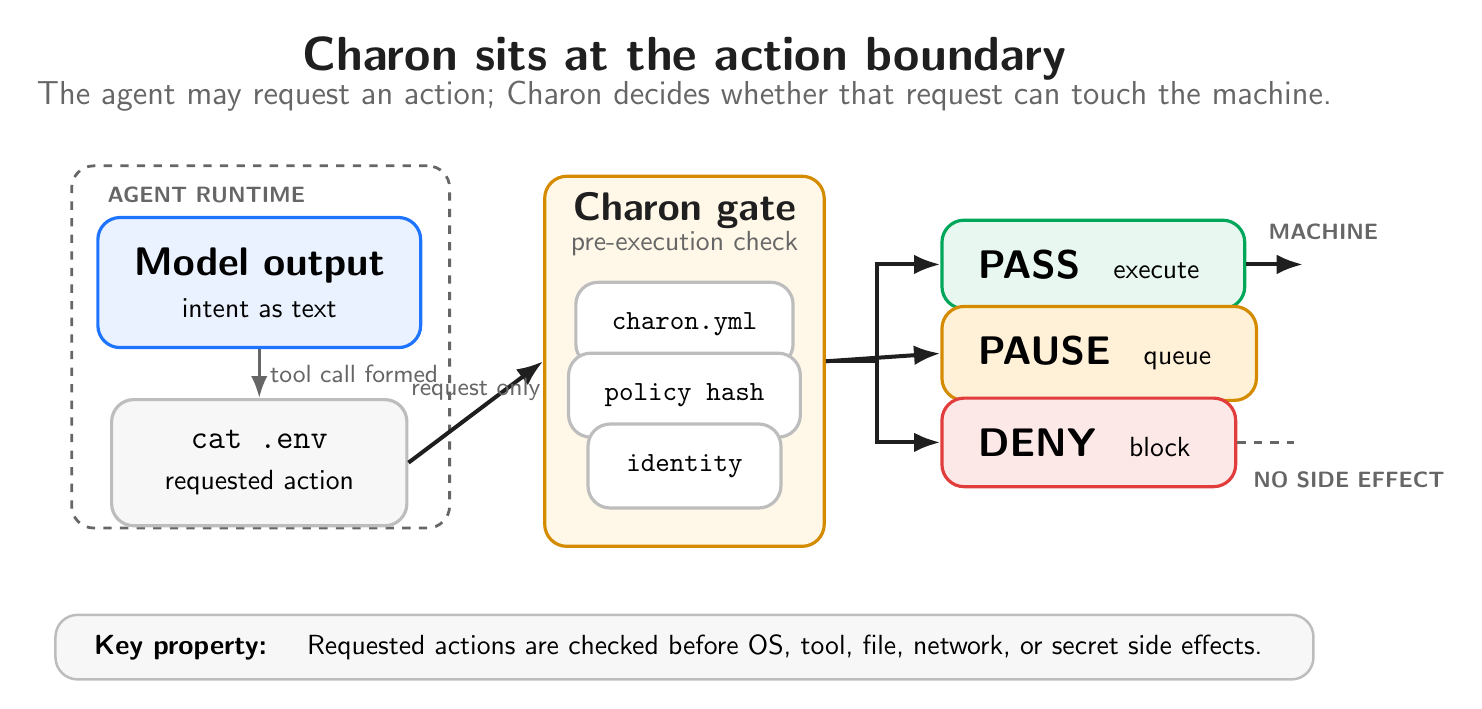
\begin{tikzpicture}[
  font=\sffamily,
  >=Latex,
  node distance=0,
  box/.style 2 args={
    draw=#1,
    fill=#2,
    rounded corners=8pt,
    line width=1.15pt,
    align=center,
    inner xsep=13pt,
    inner ysep=11pt
  },
  flow/.style={->, line width=1.45pt, draw=ink},
  softflow/.style={->, line width=1.1pt, draw=muted},
  noflow/.style={line width=1.1pt, draw=muted, dashed},
  tag/.style={font=\sffamily\bfseries\footnotesize, text=muted},
  title/.style={font=\sffamily\bfseries\LARGE, text=ink},
  subtitle/.style={font=\sffamily\large, text=muted},
  small/.style={font=\sffamily\small, text=muted},
  code/.style={font=\ttfamily\bfseries\large, text=ink}
]

% canvas anchors
\coordinate (L) at (0,0);

% Title
\node[title] at (8.0,7.2) {Charon sits at the action boundary};
\node[subtitle] at (8.0,6.72) {The agent may request an action; Charon decides whether that request can touch the machine.};

% Agent runtime group
\node[
  draw=muted,
  dashed,
  rounded corners=8pt,
  line width=1pt,
  minimum width=4.8cm,
  minimum height=4.6cm,
  anchor=north west
] (agentbox) at (0.2,5.85) {};
\node[tag, anchor=west] at ($(agentbox.north west)+(0.35,-0.38)$) {AGENT RUNTIME};

\node[box={blueline}{bluefill}, minimum width=3.75cm, minimum height=1.1cm] (model) at (2.6,4.35) {
  {\bfseries\Large Model output}\\[3pt]
  {\normalsize intent as text}
};

\node[box={grayline}{softgray}, minimum width=3.75cm, minimum height=0.95cm, below=0.62cm of model] (request) {
  {\ttfamily\bfseries\large cat .env}\\[3pt]
  {\normalsize requested action}
};

\draw[softflow] (model.south) -- node[right, small] {tool call formed} (request.north);

% Charon gate
\node[box={gateline}{gatefill}, minimum width=3.55cm, minimum height=4.7cm] (gate) at (8.0,3.35) {};
\node[font=\sffamily\bfseries\Large, text=ink] at ($(gate.north)+(0,-0.45)$) {Charon gate};
\node[font=\sffamily\normalsize, text=muted] at ($(gate.north)+(0,-0.88)$) {pre-execution check};

\node[box={grayline}{white}, minimum width=2.45cm, minimum height=0.52cm] (policy) at (8.0,3.82) {{\ttfamily\bfseries charon.yml}};
\node[box={grayline}{white}, minimum width=2.45cm, minimum height=0.52cm] (hash) at (8.0,2.92) {{\ttfamily\bfseries policy hash}};
\node[box={grayline}{white}, minimum width=2.45cm, minimum height=0.52cm] (identity) at (8.0,2.02) {{\ttfamily\bfseries identity}};

% Request arrow
\draw[flow] (request.east) -- node[above, small] {request only} (gate.west);

% Verdict boxes
\node[box={passline}{passfill}, minimum width=3.15cm, minimum height=0.78cm, anchor=west] (pass) at (11.25,4.58) {
  {\bfseries\Large PASS}\hspace{0.42cm}{\normalsize execute}
};
\node[box={gateline}{pausefill}, minimum width=3.15cm, minimum height=0.78cm, anchor=west] (pause) at (11.25,3.45) {
  {\bfseries\Large PAUSE}\hspace{0.42cm}{\normalsize queue}
};
\node[box={denyline}{denyfill}, minimum width=3.15cm, minimum height=0.78cm, anchor=west] (deny) at (11.25,2.32) {
  {\bfseries\Large DENY}\hspace{0.42cm}{\normalsize block}
};

% Verdict fan-out
\draw[flow] (gate.east) -- ++(0.65,0) |- (pass.west);
\draw[flow] (gate.east) -- (pause.west);
\draw[flow] (gate.east) -- ++(0.65,0) |- (deny.west);

% Machine / no side effect
\draw[flow] (pass.east) -- ++(0.72,0);
\node[tag, anchor=west] at ($(pass.east)+(0.16,0.42)$) {MACHINE};
\draw[noflow] (deny.east) -- ++(0.72,0);
\node[tag, anchor=west] at ($(deny.east)+(0.08,-0.48)$) {NO SIDE EFFECT};

% Key property
\node[
  draw=grayline,
  fill=softgray,
  rounded corners=8pt,
  line width=0.9pt,
  minimum width=12.35cm,
  minimum height=0.82cm,
  align=left,
  inner xsep=14pt
] at (8.0,-0.28) {
  {\bfseries Key property:} \quad Requested actions are checked before OS, tool, file, network, or secret side effects.
};

\end{tikzpicture}
\end{document}
